\documentclass{article}
\usepackage[a4paper, total={6in, 8in}]{geometry}
\usepackage{fontenc}
\usepackage[ngerman]{babel}
\usepackage[utf8]{inputenc}
\usepackage{graphicx}
\usepackage{caption}
	\DeclareCaptionLabelFormat{abbrev}{Abb. #2}
	\captionsetup[figure]{labelformat=abbrev, font=it}
\usepackage{subcaption}
%\usepackage{wrapfig}
\usepackage{grffile}
\usepackage{subcaption}
\usepackage[export]{adjustbox}
\graphicspath{ {../pics/Blatt_4} }
\usepackage{alphalph}
\usepackage{amsmath}
\DeclareUnicodeCharacter{2028}{\linebreak}
\usepackage{hyperref}
\usepackage{listings}
\usepackage{color}
\usepackage{multicol}
\setlength{\columnsep}{1cm}



\definecolor{dkgreen}{rgb}{0,0.6,0}
\definecolor{gray}{rgb}{0.5,0.5,0.5}
\definecolor{mauve}{rgb}{0.58,0,0.82}

\lstset{frame=tb,
  language=Java,
  aboveskip=3mm,
  belowskip=3mm,
  showstringspaces=false,
  columns=flexible,
  basicstyle={\small\ttfamily},
  numbers=left,
  numberstyle=\tiny\color{gray},
  keywordstyle=\color{blue},
  commentstyle=\color{dkgreen},
  stringstyle=\color{mauve},
  breaklines=true,
  breakatwhitespace=true,
  tabsize=3
}
\usepackage{datetime}
\newdateformat{myformat}{\THEDAY{ten }\monthname[\THEMONTH], \THEYEAR}

\begin{document}
		\begin{titlepage}
		\centering
		{\scshape\LARGE
			Ereignisdiskrete Systeme
			\par}
		\vspace{1.5cm}
		{\huge\bfseries Praktikum Blatt 4 - Stateflow\par}
		\vspace{1.5cm}
		{\LARGE\itshape Jan Kristel, Alexandra Moritz\par}
		\vfill
			Aufsicht von Frau Rembold\par
			
		\vfill	
			{\large \today \par}	
		
	\end{titlepage}
	
	\tableofcontents
	\clearpage
\newpage
	\begin{multicols}{2}
	\section{Was ist \textbf{Stateflow} ?}
		\renewcommand{\thesubsection}{\alph{subsection})}
		\subsection{Was ist Stateflow?}
			Stateflow ist eine grafische Erweiterung von Simulink zur Modellierung und Simulation von
			\begin{itemize}
				\item Ereignisgesteuerten reaktiven Systemen mit endlich vielen Zuständen
				\item Zustandsautomaten (engl.: Finite State Machines)
			\end{itemize}
			Zustandsmaschinen sind ein Konzept aus der Informatik und der Systemtheorie, das verwendet wird, um das Verhalten eines Systems oder einer Komponente zu modellieren, das sich in verschiedenen Zuständen befinden kann.
			Es lassen sich Zustandsdiagramme erstellen, bestehend aus Zuständen, Übergängen zwischen diesen und Aktionen, die bei den Übergängen ausgeführt werden. Diese Diagramme beschreiben das Verhalten eines Systems. 
			\begin{itemize}
				\item Zustände repräsentieren, die verschiedenen Phasen oder Modi, in denen sich ein System befinden kann.
				\item Übergänge zeigen die Bedingungen an, unter denen das System von einem Zustand in einen anderen wechselt. 
				\item Aktionen definieren die Operationen oder Reaktionen, die beim Zustandsübergang ausgeführt werden sollen.
			\end{itemize} 
			In Kombination mit MATLAB und Simulink wird Stateflow verwendet, um das Verhalten von komplexen Systemen zu modellieren und zu simulieren.
			 Dabei wird die Integration von Zustandsmaschinen in die allgemeine Systemmodellierung und -simulation ermöglicht und eine visuelle Darstellung des Systemverhaltens geboten.
			Entwickler bekommen eine effiziente Methode zur Modellierung und Implementierung von komplexen Systemverhalten.
		\subsection{Was ist ein/e ...}
			\subsubsection{Chart?}
				Zustandsautomaten werden als Zustandsübergangsdiagramme, s.g. \textbf{Charts} dargestellt. 
		\end{multicols}
			\begin{figure}[hb]
				\begin{subfigure}{0.5 \textwidth}
					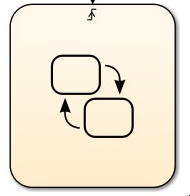
\includegraphics[scale=0.8]{Chart_extern.png}
					\caption{Darstellung eines Charts von ''außen'' aus dem Simulinkeditor}
					\label{fig_1:Chart extern}
				\end{subfigure}
				\begin{subfigure}{0.5 \textwidth}
					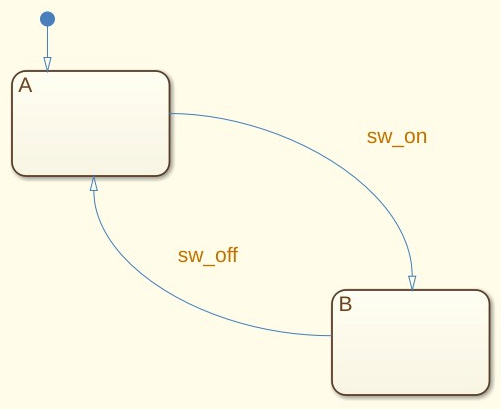
\includegraphics[scale=0.4]{Chart_intern.png}
					\caption{Darstellung eines Chart von ''innen''.}
					\label{fig_2: Chart intern}
				\end{subfigure}
			\end{figure}
		\begin{multicols}{2}
		\renewcommand{\thesubsection}{\alph{subsection})}
				Es besteht aus verschiedenen Zuständen, Übergängen, Aktionen und Ereignisse.
				Dabei kann ein Chart auch hierarchisch organisiert sein, wobei ein \textit{übergeordneter Chart mehrere Untercharts enthalten kann}. Diese Hierarchie ermöglicht es, komplexe Systeme in kleinere und besser handhabbare Teile zu zerlegen.
				In einem Chart können auch Aktionen definiert werden, die beim Eintritt oder Verlassen eines Zustands auszuführen sind. Beispielsweise Berechnungen, Signalmanipulationen oder das Auslösen von Ereignissen.
 				Durch die Verwendung von Charts ist es möglich komplexe Systeme auf intuitive Weise zu modellieren und zu verstehen. Charts bieten eine visuelle Darstellung des Systemverhaltens und ermöglichen es Entwicklern, den Zustandsfluss und die Interaktionen zwischen den Zuständen effizient zu entwerfen und zu analysieren.
			\subsubsection{State?}
				Ein \textbf{State} repräsentiert einen bestimmten Zustand in dem sich ein System befindet. Dieser ist definiert durch eine eindeutige Kombination von Eigenschaften, die das Verhalten und die Merkmale des Systems zu einem bestimmten/dem aktuellekn Zeitpunkt beschreiben. 
				Der State kann als eine Art Container betrachtet werden, der Aktionen, Übergänge und interne Variablen enthält (ähnlich dem Chart).
				Jeder State kann eine oder mehrere der folgenden Eigenschaften haben:
				\begin{itemize}
					\item \textbf{Aktionsblöcke} enthalten den auszuführenden Code/Aktionen, wenn der Zustand aktiv ist. Diese können \textit{Berechnungen, Signalmanipulationen, Funktionsaufrufe oder andere spezifische Operationen} umfassen.
					\item \textbf{Übergänge} beschreiben den Wechsel von einem Zustand in einen anderen, unter bestimmten Bedingungen. Diese Bedingungen können auf Ereignissen, bool'schen Bedingungen oder zeitlichen Auslösern basieren.
					\item \textbf{Eingangsereignisse} werden von States empfangen, die von externen Quellen oder anderen Zuständen generiert werden. Diese Ereignisse können den Zustandsübergang oder das Verhalten im Zustand beeinflussen.
					\item \textbf{aktive Dauer} gibt an, wie lange der Zustand aktiv bleibt, bevor ein Übergang zu einem anderen Zustand ausgelöst wird.
				\end{itemize}
			\subsubsection{History Junction?}
				Ein \textbf{History Junction} ermöglicht es, den Zustand eines übergeordneten States zu speichern und beim erneuten Eintritt in diesen an der Stelle fortzufahren, an der er zuvor verlassen wurde. Es stellt eine Möglichkeit der Wiederherstellung dar, anstatt immer wieder von Anfang an zu beginnen.
				%Normalerweise erfolgt der Zustandsübergang in Stateflow von einem Zustand zum nächsten gemäß definierten Bedingungen. Beim Verlassen eines Zustands gehen alle internen Zustände und deren Zustandsverlauf verloren. In manchen Fällen kann es jedoch wünschenswert sein, den vorherigen Zustand fortzusetzen, wenn ein übergeordneter Zustand erneut betreten wird.
				%Hier kommt das Konzept des History JuncDons ins Spiel. Ein History JuncDon ist eine spezielle Art von Übergang in einem Zustandsautomaten. Wenn ein Zustand einen History JuncDon-Übergang besitzt und der übergeordnete Zustand erneut betreten wird, überprüM Stateflow, ob ein vorheriger Zustand gespeichert wurde. Wenn ja, wird der Zustand an dieser Stelle fortgesetzt, ansta* vom Anfang zu beginnen. Dadurch wird der vorherige Zustand wiederhergestellt.
				%Die Verwendung eines History JuncDons ermöglicht es, den Zustandsverlauf beizubehalten und das Verhalten eines Systems an der Stelle wieder aufzunehmen, an der es zuvor unterbrochen wurde. Dies kann insbesondere dann nützlich sein, wenn der Zustandsverlauf oder der Systemkontext wichDg sind und nicht bei jedem Eintri* in den übergeordneten Zustand verloren gehen sollen.
			\subsubsection{Default Transition?}
				Ein \textbf{Default Transition} ist eine Art Übergang in einem Zustandsautomaten, der ausgelöst wird, wenn keine anderen Übergänge die spezifischen Bedingungen erfüllen. Die Default Transition wird genutzt, um einen \textit{Standardpfad} zu definieren, der genommen wird, wenn keine anderen Übergänge aktiviert werden können.
				%In einem Stateflow-Chart kann ein Zustand mehrere ausgehende Übergänge haben, die durch Bedingungen oder Ereignisse ausgelöst werden. Wenn keiner dieser Übergänge aktiviert wird, wird der Default Transition aktiviert und der Zustand wechselt entsprechend zu einem anderen Zustand.
				Sie ist \textit{optional und muss nicht in jedem Zustand definiert werden}. Wenn jedoch eine Default Transition in einem Zustand vorhanden ist und keine anderen Übergänge aktiviert werden, erfolgt der Zustandsübergang entsprechend dieser.
				%Der Default Transition kann als eine Art "Fallback" betrachtet werden, um sicherzustellen, dass der Zustand des Systems in einen anderen Zustand wechselt, auch wenn keine spezifischen Bedingungen erfüllt sind. Es bietet eine Möglichkeit, das Verhalten des Systems zu steuern, wenn keine anderen Übergänge aktiviert werden können.
				Bei der Modellierung mit Stateflow ist es wichtig, die Verwendung von Default Transitions sorgfältig zu planen und zu überprüfen, um sicherzustellen, dass das Verhalten des Systems den Anforderungen und Spezifikationen entspricht.
			\subsubsection{Connective Junction?}
				Ein \textbf{Connective Junction} ermöglicht die Verbindung von mehreren ausgehenden Übergängen aus einem Zustand zu einem einzelnen Zielzustand.
				Normalerweise können in einem Zustand mehrere ausgehende Übergänge zu verschiedenen Zielzuständen definiert werden. Bei Verwendung einer Connective Junction können diese Übergänge an einem einzigen Verbindungspunkt zusammengeführt werden, bevor sie den Zielzustand erreichen.
				%Die Connective Junction dient als Zwischenschritt, um mehrere Übergänge zu gruppieren und den Übergangsausgangspunkt in einem Zustand zu konsolidieren. Sie ermöglicht es, die Ausführung von Aktionen oder die Bedingungsüberprüfung an einem einzigen Ort zu zentralisieren, bevor der endgültige Zustandswechsel stattfindet.
			\subsubsection{Truth Table}
				Eine \textbf{Wahrheitstabelle} ist eine tabellarische Darstelliung von logischen Zuständen. Dabei erfüllt diese folgende Eigenschaften:
				\begin{itemize}
					\item Vermeidung von unübersichtlichen UND/ODER-Verknüpfungen
					\item wird wie grafische Funktionen verwendet
					\item enthält
					\begin{itemize}
						\item Funktionsprototypen 
						\item Condition-Table
						\item Decision-Table
					\end{itemize}
				\end{itemize}
				D.h. jede Spalte $D_i$ entspricht einer IF-Bedingung, jede Zeile ist eine UND-Verknüpfungen aller Bedingungen in einer Spalte.
				Die Aktion der ersten wahren Spalte (von links nach rechts) wird ausgeführt (und dann das Truth Table sofort verlassen)
			\subsubsection{Function ?}
				Eine \textbf{Funktion} repräsentiert einen blockartigen Container, der eine Gruppe von Aktionen oder Berechnungen enthält. Dieser wird verwendet, um komplexe Logik zu organisieren und \textit{wiederverwendbaren Code} zu erstellen.
				Die Funktion bzw. der Block kann eine beliebige Anzahl von Ein- und Ausgabeparametern haben. Die enthaltenen Aktionen können ausgeführt, Variablen deklariert, Berechnungen durchgeführt, Bedingungen überprüft, Zustände geändert und andere Funktionen aufgerufen werden.\\
				Funktionen können in einem Zustandsdiagramm oder in anderen Funktionen verwendet werden.
			\subsubsection{Embedded MATLAB Function ?}
				Bei \textbf{Embedded functions} handelt es sich um Funktionen, die \textit{innerhalb einer anderen Funktion} definiert sind. Im Gegensatz zu separaten, eigenständigen Funktionen sind eingebettete Funktionen eng mit der umgebenden Funktion verbunden und haben \textit{Zugriff auf deren Variablen und Parameter}.
				Ihre Verwendung bietet mehrere Vorteile:
				\begin{itemize}
					\item Modulare Programmierung
					\item Vermeidung von Namenskonflikten: \\Eingebettete Funktionen haben einen begrenzten Scope und können Variablennamen verwenden, die in der umgebenden Funktion bereits vorhanden sind, ohne Konflikte zu verursachen. Dadurch können lokale Variablen effektiv verwendet werden, ohne den globalen Namensraum zu beeinträchtigen.
					\item Datensicherheit: \\Die Trennung des Gültigkeitsbereichs der eingebetteten Funktionen und dem restliche Namensraum bezüglich der Variablen (lokal bzw. global) bietet eine gewisse Datensicherheit und verhindert unerwünschte Seiteneffekte oder Änderungen an den Variablen von außen.
				\end{itemize}
			%Eingebettete Funktionen sind ein Feature in bestimmten Programmiersprachen wie MATLAB. Sie ermöglichen eine effektive und strukturierte Programmierung, insbesondere für komplexe Funktionen oder Algorithmen, die in kleinere, wiederverwendbare Teile aufgeteilt werden können.
			\subsubsection{Box ?}
				Zustände und Funktionen werden in rechteckigen Boxen dargestellt. Eine \textbf{Zustandsbox} repräsentiert einen State im Zustandsdiagramm, während eine \textbf{Funktionsbox} eine Funktion innerhalb diesem darstellt. Diese Boxen enthalten Logik, Aktionen und Transitionen, die den Zustandsautomaten steuern.
				Boxen sind grafische Einheiten zur visuellen Organisation eines Charts. Sie dienen dabei:
				\begin{itemize}
					\item der Zusammenfassung von beliebigen grafischen Elementen um Charts übersichtlicher zu machen.
					\item haben keinen Einfluss auf Funktionen des Modells
					\item können Einfluss nehmen auf die Aufführungsreihenfolge:
					\begin{itemize}
						\item von oben nach unten
						\item von links nach rechts (ähnlich wie bei parallelen Superstates)
					\end{itemize}
				\end{itemize} 
		\subsection{Wie wird der grafische Editor gestartet?}
			\begin{itemize}
				\item Öffnen eines Simulink-Modell: Lade das gewünschte Simulink-Modell, in dem du Stateflow verwenden möchtest, oder erstelle ein neues Modell.
				\item Öffnen des Stateflow-Editors: Im Reiter Modelling, sieht man eine Palette mit verschiedenen Simulink-Blöcken. Hier wählt man \textbf{Insert Chart}. Oder über den Libray Browser den Abschnitt Stateflow finden und den Chart-Block in das Modell ziehen.
				\item Doppelklick auf den Stateflow-/Chart-Block
				\item Danach wird der grafische Editor für Stateflow geöffnet. Hier können Zustandsdiagramme erstellt, Zustandsübergänge definiert und die Logik des Stateflow-Modells gestaltet werden.
			\end{itemize}
		\subsection{Was ist der Model Explorer?}
			Es handelt sich um ein interaktives Fenster, das es ermöglicht, auf eine strukturierte und übersichtliche Weise auf verschiedene Elemente eines Simulink-Modells zuzugreifen und diese zu verwalten. Er bietet eine alternative Sicht auf das Modell und erleichtert die Navigation, Inspektion und Bearbeitung der Modellkomponenten.
			Einige Funktionen sind:
			\begin{itemize}
				\item Hierarchische Darstellung: \\Das Simulink-Modell wird in einer hierarchischen Struktur angezeigt. Es ermöglicht das Ausklappen/Zusammenklappen von Komponenten, um eine bessere Übersicht und Navigation zu ermöglichen.
				\item Elementinspektion: \\Durch Auswahl eines bestimmten Modell- oder Subsystemelements können detaillierte Informationen zu diesem Element angezeigt werden. Es bietet einen schnellen Zugriff auf die Parameter, Eigenschaften und Einstellungen des ausgewählten Elements.
				\item Verknüpfungen und Referenzen: \\Der Model Explorer zeigt die Verknüpfungen und Referenzen zwischen verschiedenen Modellkomponenten an. Dadurch können Abhängigkeiten und Beziehungen zwischen den Elementen visualisiert und verwaltet werden.
				\item Such- und Filterfunktionen: \\Mit diesen könne bestimmte Modellkomponenten basierend auf Namen, Typen oder anderen Kriterien gefunden werden können. Dies erleichtert die Suche in großen und komplexen Modellen.
				\item Modifikationen und Aktualisierungen: \\Es ist wird das Hinzufügen, Umbenennen, Löschen und Aktualisieren von Modellkomponenten ermöglicht. Dadurch können Modelländerungen schnell und einfach vorgenommen werden, ohne den grafischen Editor zu öffnen.
			\end{itemize}
		\subsection{Wie werden einem Chart oder State Daten bzw. Events zugewiesen?}
			\begin{itemize}
				\item Öffne den Stateflow-Editor: \\Öffne den Stateflow-Editor, indem du doppelt auf den entsprechenden Chart-Block oder State-Block im Simulink-Modell klickst.
				\item Definiere Eingänge: \\Im Stateflow-Editor kannst du Eingänge für den Chart oder State definieren. Klicke mit der rechten Maustaste auf den Chart-Block oder State-Block und wähle ''Properties'' oder ''Eigenschaften'' aus, um die Eigenschaften des Blocks anzuzeigen.
				\item Weise Eingänge zu: \\In den Eigenschaften des Charts oder States können Eingänge definieret werden. Klicke auf den Reiter ''Inputs'' oder ''Eingänge'' und füge die gewünschten Eingänge hinzu. Hier könne sie benannt und ihren Datentyp festgelegt werden.
				\item Verwende Eingänge in Transitionen oder Aktionen: \\Sobald die Eingänge definiert sind, können sie in Transitionen oder Aktionen des Charts oder States verwendet werden. In einer Transition kann eine Bedingung, dargestellt durch \textbf{eckige Klammern}, festgelegt werden, die den Wert des Eingangs prüft, um den Zustandsübergang auszulösen. In Aktionen, dargestellt durch \textbf{geschweifte Klammern}, kann der Wert des Eingangs lesen und damit Berechnungen durchführen oder Zustandslogik steuern.
				\item Aktualisiere das Simulink-Modell: \\Nachdem Eingänge zugewiesen und verwendet wurden, speichert man den Stateflow-Editor und aktualisiertdas Simulink-Modells. Dadurch werden die Änderungen übernommen und das Modell ist bereit, Daten bzw. Events über die definierten Eingänge zu empfangen und zu verarbeiten.
				\item Durch die Zuweisung von Eingängen können Charts und States in Stateflow mit Daten bzw. Events interagieren und entsprechend reagieren. Es ermöglicht die flexible Steuerung des Zustandsverhaltens basierend auf externen Ereignissen oder Datenänderungen.
			\end{itemize}
		\subsection{Wie werden im Chart Kommentare eingefügt ?}
		\begin{itemize}
			\item Wähle das Tool ''Comment'' aus: \\Im Stateflow-Editor findet man in der Symbolleiste verschiedene Tools und Symbole. Klicke auf das ''Comment''-Symbol, das oft wie ein Sprechblasensymbol aussieht. Alternativ kannst du die Tastenkombination ''Ctrl+Alt+C'' verwenden.
			\item das Kommentar-Symbol in den Chart ziehen: \\Nachdem das ''Comment''-Tool ausgewählt ist, folgt dem Zeiger ein Kommentarsymbol. Mit Mausklick kann jetzt ein Fenster gezogen werden. Die Größe des Fenster gibt die Größe des Kommentars vor.
			\item den Kommentar schreiben: \\Sobald das Kommentar-Symbol platziert ist, wird ein Textfeld geöffnet, in dem der Kommentar eingegeben werden kann.
		\end{itemize}
		\subsection{Was bedeutet in Stateflow ''Exclusiv'' und ''Parallel'' ?}
			\subsubsection{Exclusiv}
				\paragraph{Exklusive Verbindung:}
					 Im Kontext von Zustandsübergängen bedeutet ''exklusiv'', dass nur ein einzelner Übergang zu einem bestimmten Zeitpunkt aktiv sein kann. Wenn mehrere Übergänge gleichzeitig aktiviert werden könnten, wird der Übergang mit der höchsten Priorität oder den spezifischsten Bedingungen ausgeführt.
				\paragraph{Exklusiver Zustand:}
					Ein exklusiver Zustand bezeichnet einen Zustand, der einen bestimmten Satz von Aktivitäten oder Aktionen ausführt, solange er aktiv ist. Andere Zustände im gleichen Zustandsdiagramm bleiben in diesem Fall deaktiviert.
			\subsubsection{Parallel}
				\paragraph{Parallele Aktivität:} Im Kontext von Zuständen ermöglicht der parallele Verbindungstyp die gleichzeitige Aktivierung mehrerer Zustände. Dadurch können mehrere Aktivitäten oder Aktionen parallel ablaufen. Parallele Aktivitäten können entweder explizit als parallele Zustände im Zustandsdiagramm modelliert werden oder durch die Verwendung von Junctions oder inneren Transitionen erreicht werden.
				\paragraph{Paralleler Zustand:} Ein paralleler Zustand bezieht sich auf einen Zustand, der parallel zu anderen Zuständen aktiv sein kann. Dadurch können mehrere parallele Aktivitäten innerhalb des Modells stattfinden. Parallele Zustände können in Stateflow-Modellen verwendet werden, um komplexes Verhalten zu modellieren, das gleichzeitig oder unabhängig voneinander ablaufen kann.\\
\newline
				Es ist wichtig zu beachten, dass die genaue Bedeutung von ''exklusiv'' und ''parallel'' stark vom Kontext innerhalb des Stateflow-Modells abhängt. Die Verwendung dieser Konzepte hängt von den spezifischen Anforderungen und der Modelllogik ab, die du in deinem Stateflow-Modell implementieren möchtest.
		\subsection{Wie wird ein Chart auf  ''Exclusiv'' eingestellt ?}
			In Stateflow kann ein Chart nicht explizit auf den ''Exklusiv''-Modus eingestellt werden. Der Exklusivitätsaspekt in Stateflow bezieht sich auf die Logik der Zustandsübergänge und Zustände im Chart.
			Wenn du sicherstellen möchtest, dass nur ein Übergang zu einem bestimmten Zeitpunkt aktiv ist, kannst du dies durch die richtige Definition der Bedingungen und Prioritäten der Zustandsübergänge erreichen. Die Priorität eines Übergangs kann durch die Reihenfolge der Übergänge im Zustandstisch oder durch die Verwendung von Guard-Bedingungen gesteuert werden. Der Übergang mit der höchsten Priorität oder der spezifischsten Bedingung wird aktiviert, während die anderen Übergänge inaktiv bleiben.
			Es ist wichDg, die Zustände und Übergänge in deinem Chart sorgfältig zu modellieren und sicherzustellen, dass die exklusive Logik deinen Anforderungen entspricht. Du kannst die Bedingungen und Prioritäten der Zustandsübergänge entsprechend anpassen, um sicherzustellen, dass nur der gewünschte Übergang zu einem bestimmten Zeitpunkt aktiv ist.
			Es gibt keine spezielle Einstellung oder Schalter, um den Chart selbst auf "Exklusiv" zu setzen. Die Exklusivität wird durch die Definition der Zustandsübergänge und deren Bedingungen innerhalb des Charts erreicht.
		\subsection{Was beschreibt das Label einer Transition}
			\begin{itemize}
				\item Bedingtes Label: \\Eine Transition kann ein bedingtes Label haben, das eine logische Bedingung enthält. Diese Bedingung wird evaluiert, und wenn sie wahr ist, wird der Übergang aktiviert. Ein Beispiel für ein bedingtes Label könnte $condition > 0$ sein, wobei $condition$ eine Variable oder ein Ausdruck ist, der eine numerische Bedingung repräsentiert.
				\item Event Label: \\Eine Transition kann auch ein Event Label haben, das das Auftreten eines bestimmten Ereignisses auslöst. Das Ereignis kann entweder von externen Quellen wie Sensoren oder anderen Komponenten des Systems ausgelöst werden oder innerhalb des Stateflow-Modells generiert werden. Ein Event Label kann beispielsweise $event\_name$ sein, wobei $event\_name$ der Name des Ereignisses ist.
				\item Timer Label: \\Eine Transition kann auch ein Timer Label haben, das eine Zeitverzögerung angibt, bevor der Übergang aktiviert wird. Das Timer Label kann eine Zeitdauer in Sekunden oder eine Variable enthalten, die die Zeitverzögerung repräsentiert. Ein Timer Label könnte beispielsweise $timer > 5$ sein, wobei $timer$ eine Variable ist, die die Zeit in Sekunden zählt, und der Übergang nach einer Verzögerung von mehr als $5 Sekunden$ aktiviert wird.
			\end{itemize}
		\subsection{Wie starten Sie den Debugger ?}
			\begin{itemize}
				\item Aktiviere den Debugging-Modus: \\Im Stateflow-Editor gibt es eine Symbolleiste mit verschiedenen Schaltflächen. Suche nach dem "Debugging Mode"-Symbol, das oft wie ein kleines grünes Insekt aussieht. Klicke auf diese Schaltfläche, um den Debugging-Modus zu aktivieren. Alternativ funktioniert auch die Tastenkombination "Ctrl+D" verwenden.
				\item Breakpoints setzen: \\Um den Ablauf des Modells an bestimmten Punkten anzuhalten und den Debugger zu aktivieren, setze Breakpoints an den gewünschten Stellen. Klicke dazu mit der rechten Maustaste auf den Zustand oder die Transition, an der du einen Breakpoint setzen möchtest, und wähle "Set Breakpoint" oder "Breakpoint setzen" aus dem Kontextmenü aus. Du kannst auch eine bestimmte Aktion in einer Aktionssprache oder einem MATLAB-Code mit einem Breakpoint markieren.
				\item Starte die Simualtion: \\Starte die Simulation deines Simulink-Modells. Dazu kannst du den Simulationsstart-Button in der Simulink-Oberfläche verwenden.
				\item Überwache den Debugging-Ablauf: \\Sobald die Simulation läuft und ein Breakpoint erreicht wird, stoppt die Ausführung an diesem Punkt, und der Debugger tritt in den Vordergrund. Du kannst Variablenwerte überprüfen, den Ablauf Schritt für Schritt verfolgen, den Zustand des Modells überwachen und Debugging-Aktinen durchführen, wie z.B. das Setzen von Haltepunkten, das Überwachen von Variablen oder das Verändern des Modellzustands.
			\end{itemize}
		\end{multicols}
\clearpage	
	\section{Erste Schritte in Stateflow}
		\begin{figure}[h]
			\centering
			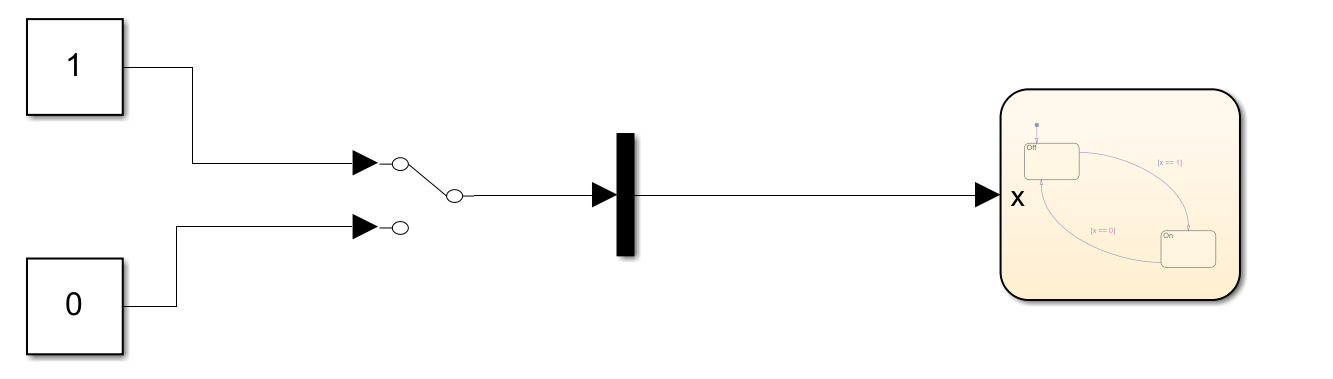
\includegraphics[scale=0.7]{Aufgabe4.2.png}
			\caption{Simulink Modell}
			\label{fig_3: Aufg_2_Simulink}
		\end{figure}
		\begin{figure}[h]
			\centering
			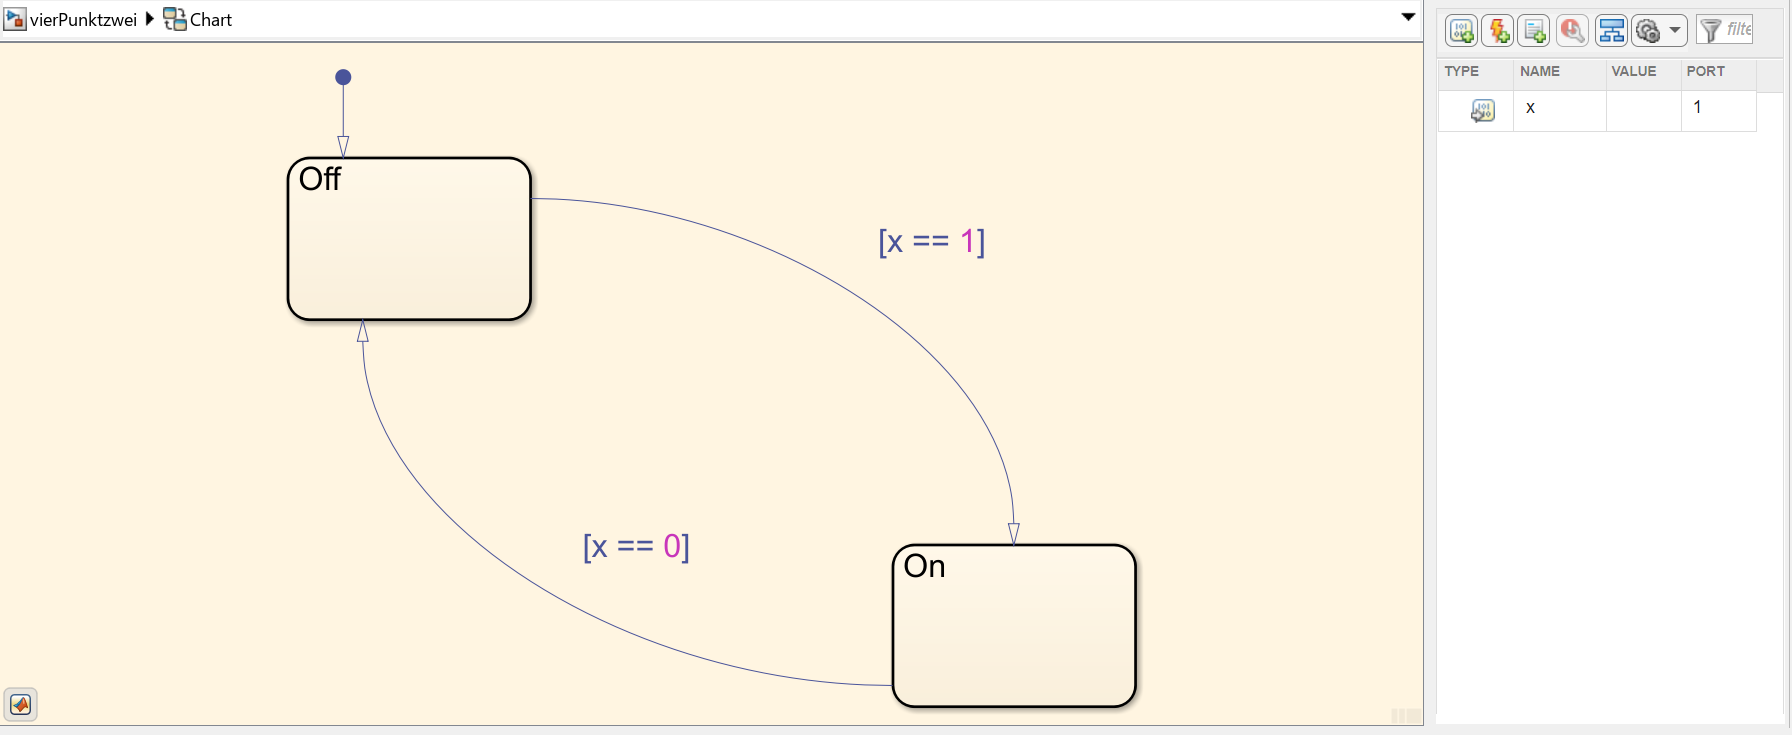
\includegraphics[scale=0.55]{Aufgabe4.2Chart.png}
			\caption{Innenansicht des Stateflow Charts.}
			\label{fig_4: ufg_2_Chart}
		\end{figure}
		Rechts in Abb.4 ist die Tabelle mit den Variablen zu sehen. Da in diesem Chart nur eine, $x$, verwendet wird, sieht die Tabelle dementsprechend klein aus. \\
		\begin{center}
			\begin{tabular}{| c | c | c | c |}
				\hline
				Type & Name & Value & Port\\
				\hline \hline
				Inputdate & x & - & 1\\
				\hline
			\end{tabular}
		\end{center}	
\clearpage
\newpage
	\section{Weitere Schritte mit Stateflow}
		\renewcommand{\thesubsection}{\alph{subsection})}
		Für die beiden Teilaufgaben \textit{a)} und \textit{b)} wird das Simulink-Modell die Form aus Abb.5 beibehalten. Hier wird beschränken sich die Änderung auf das Stateflow-Chart selbst.
			\begin{figure}[h]
				\centering
				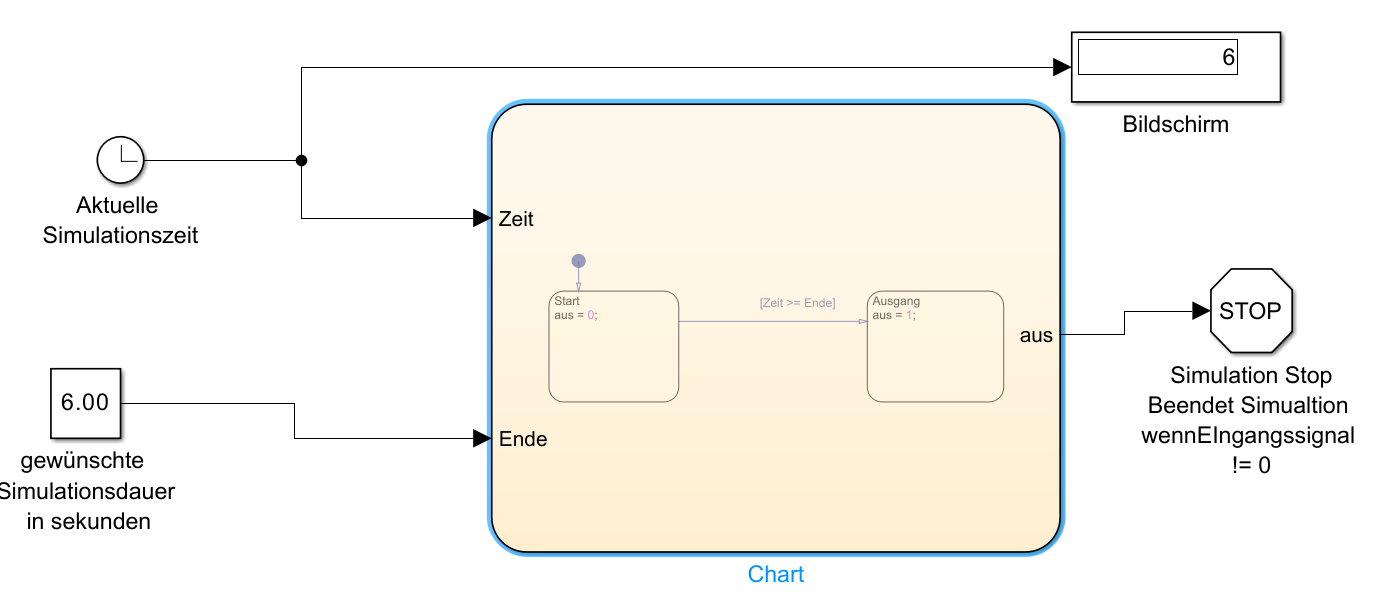
\includegraphics[scale=0.6]{Aufgabe4.3a.png}
				\caption{}
				\label{fig_5: Aufg_3_a}
			\end{figure}
		\subsection{}
			\begin{figure}[h]
				\centering
				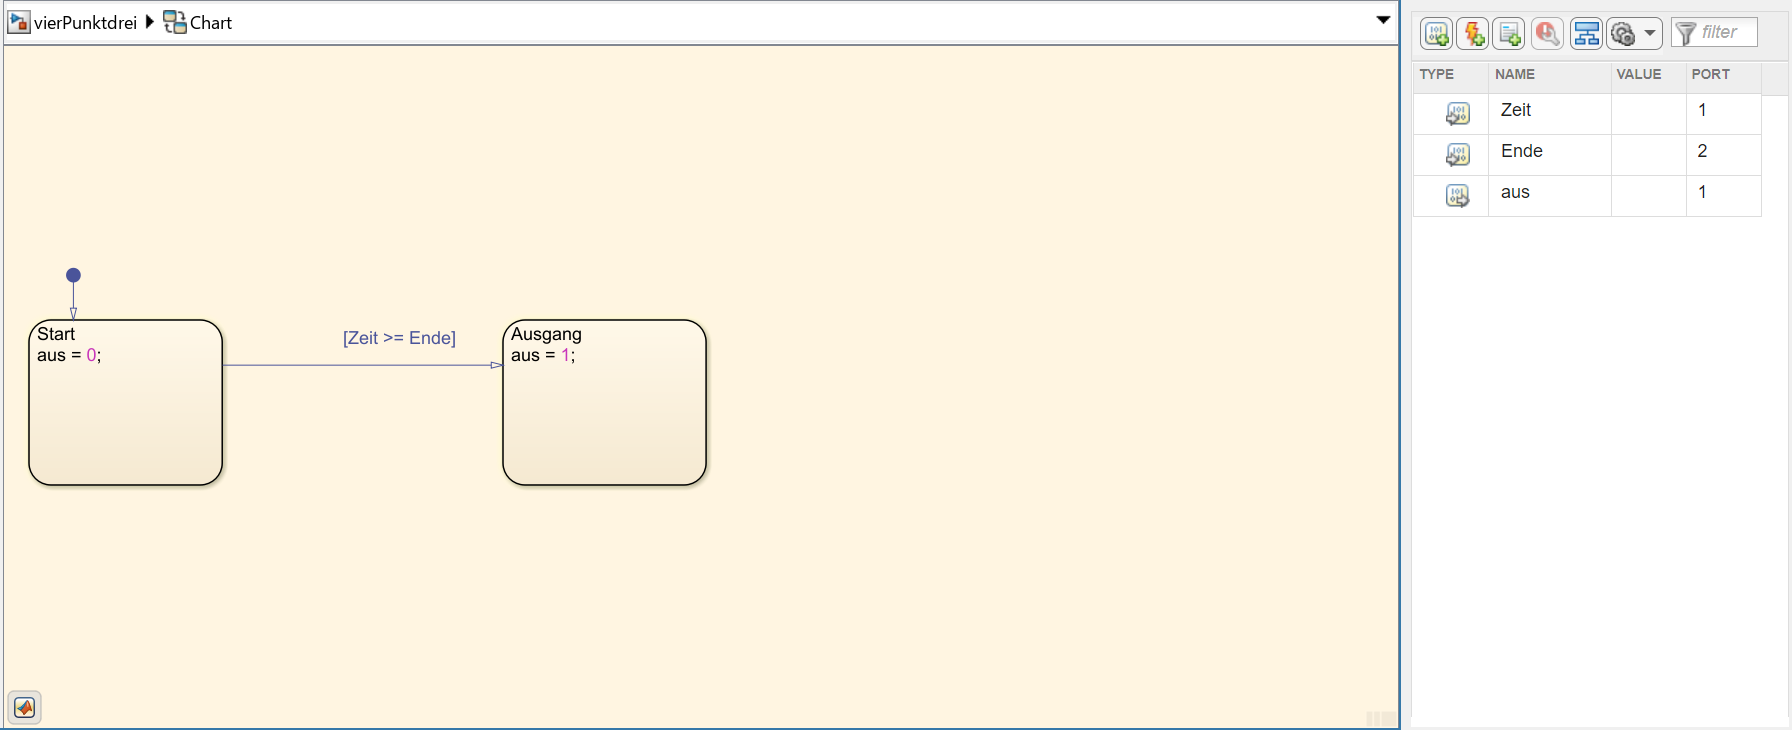
\includegraphics[scale=0.5]{Aufgabe4.3aChart.png}
				\caption{Realisiert via States.}
				\label{fig_6: Aufg_3a_Chart}
			\end{figure}
\clearpage
		\subsection{}
			\begin{figure}[h]
				\centering
				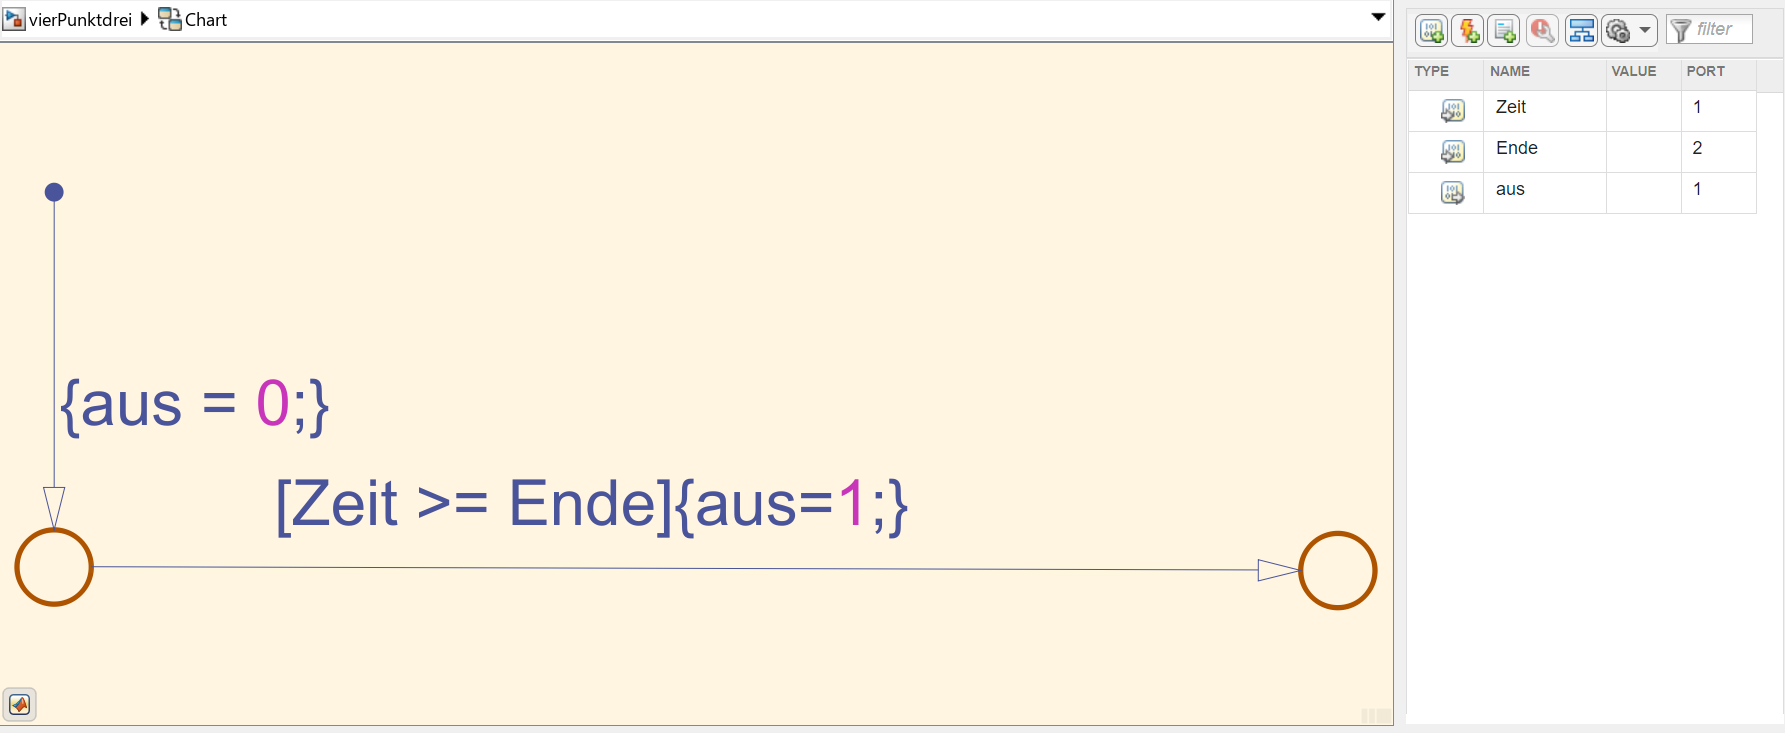
\includegraphics[scale=0.5]{Aufgabe4.3bChart.png}
				\caption{Realisiert via Junctions.}
				\label{fig_7: Aufg_3b_Chart}
			\end{figure}
		\subsection{}
			\begin{figure}[h]
				\centering
				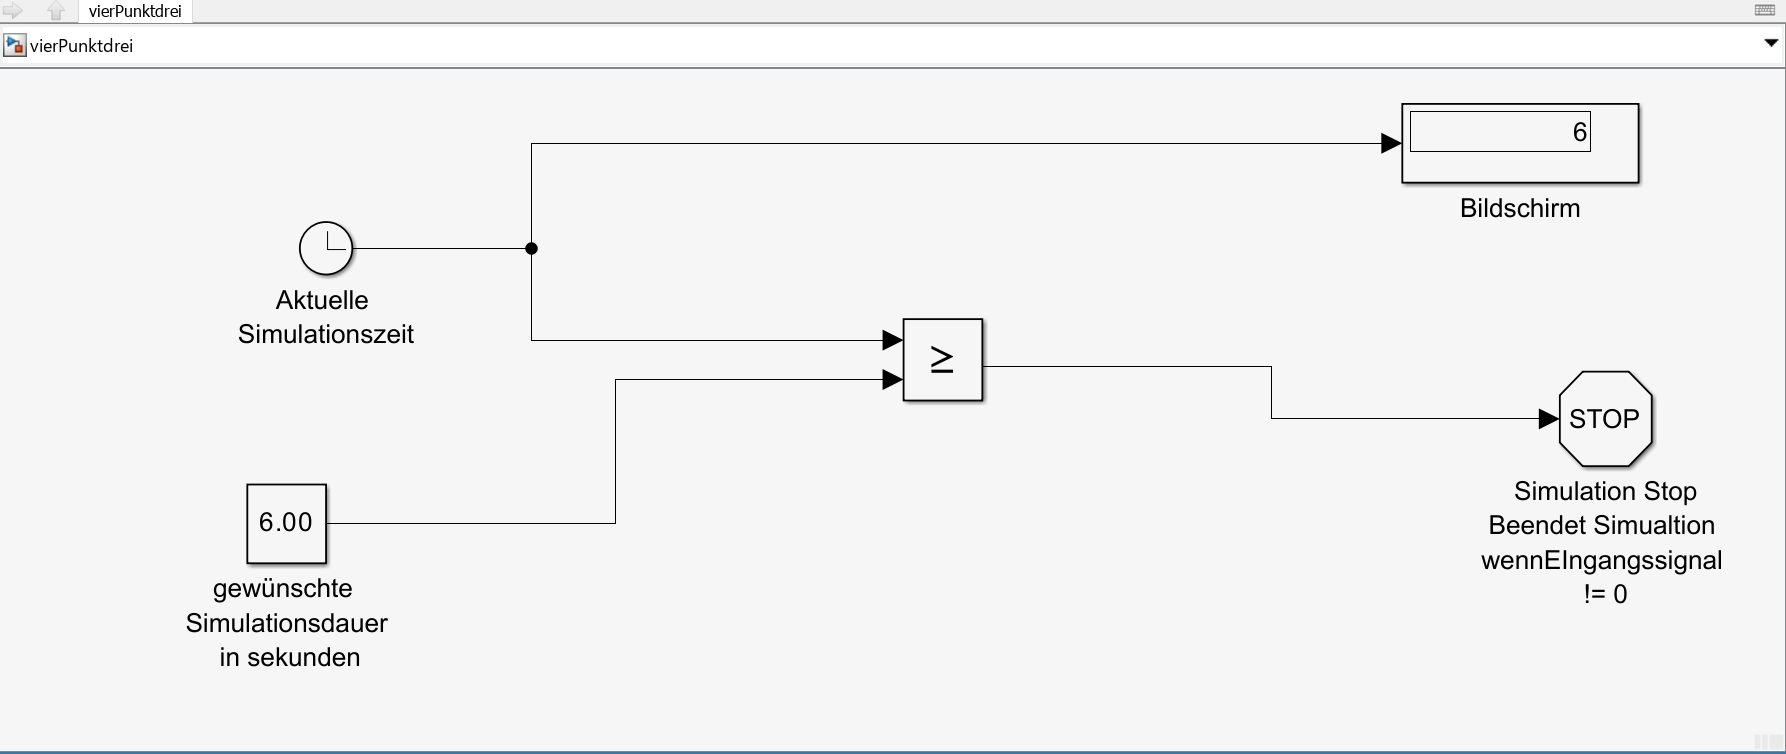
\includegraphics[scale=0.5]{Aufgabe4.3c.png}
				\caption{Realisiert durch den Simulinkblock ''Realtional Operator''.}
				\label{fig_8: Aufg_3c_Realtional_Operator}
			\end{figure}
			Durch die Realisierung mit dem Relational Operator der Simulink-Bibliothek fällt das Stateflow-Chart komplett raus.
\clearpage
		\subsection{}
			\begin{figure}[h]
				\centering
				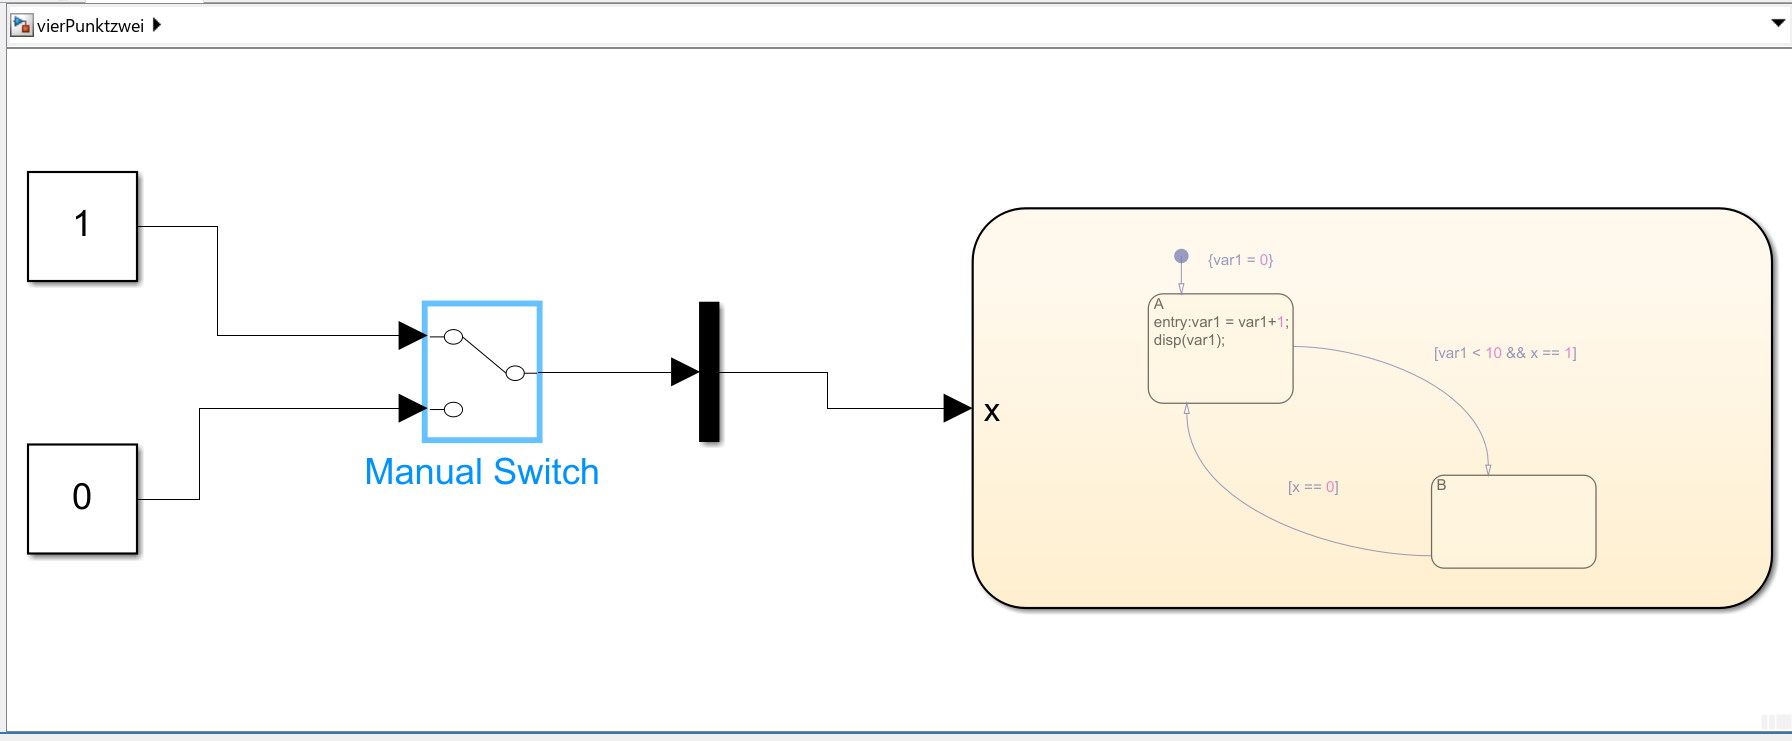
\includegraphics[scale=0.5]{Aufgabe4.3d.png}
				\caption{Von ''außen'' ist schon zu sehen, dass innerhalb des Charts mehr Informationen stehen als ursprünglich in Aufg.2 (Abb.3).}
				\label{fig_9: Aufg_3d}
			\end{figure}
			\begin{figure}[h]
				\centering
				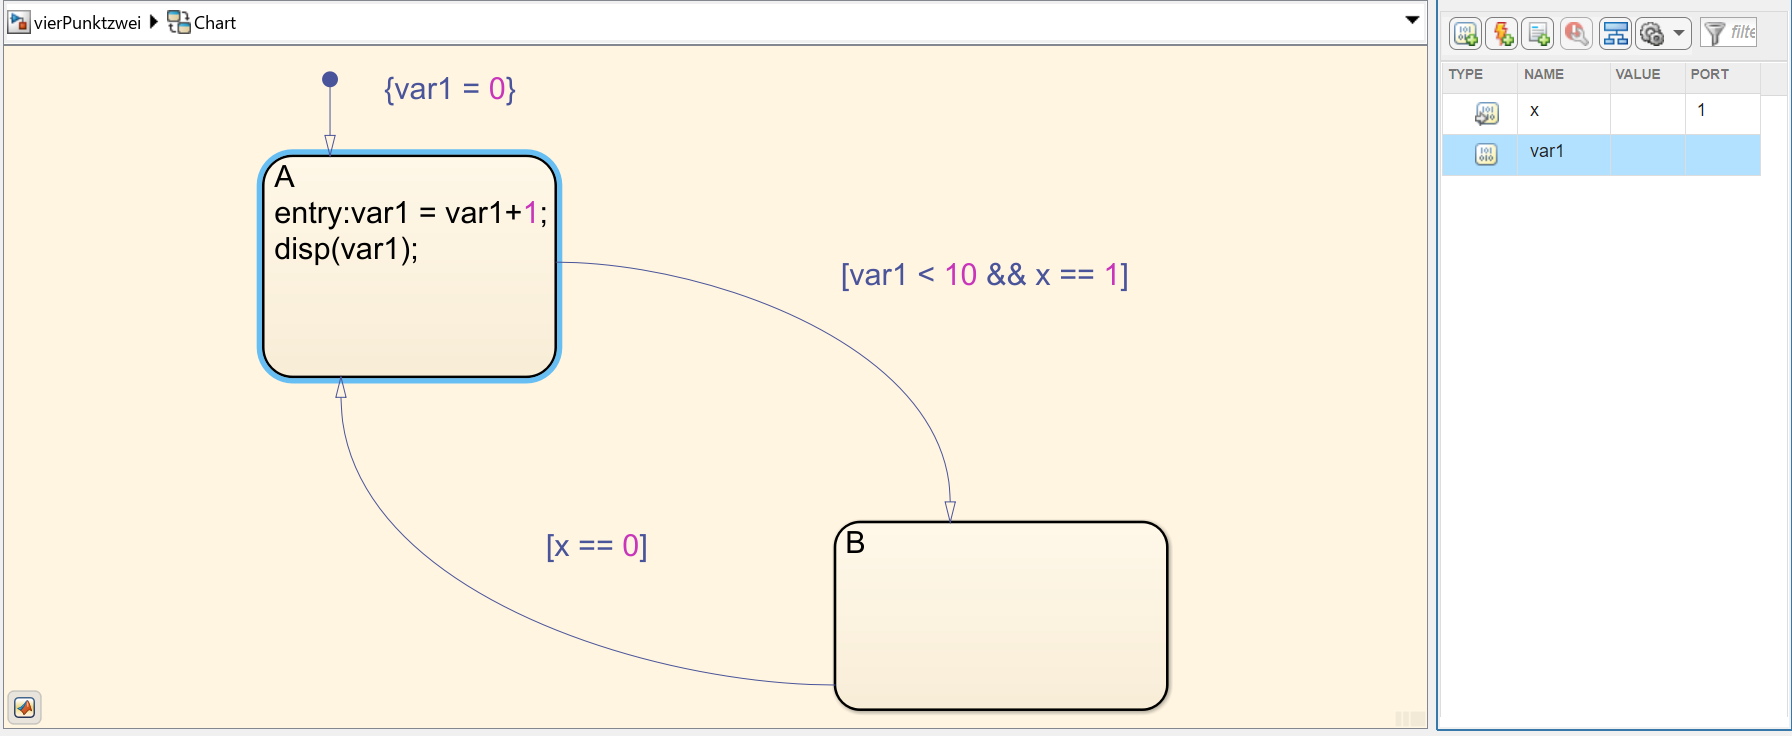
\includegraphics[scale=0.45]{Aufgabe4.3dChart.png}
				\caption{Im State A ist nun weit mehr definiert als vorher.}
				\label{fig_10: Aufg_3d_Chart}
			\end{figure}
			Den Änderungen in $State\ A$ entsprechend hat sich auch die Symboltabelle verändert.
			\begin{center}
			\begin{tabular}{| c | c | c | c |}
				\hline
				Type & Name & Value & Port\\
				\hline \hline
				InputData & x & - & 1\\
				\hline
				LocalData & var1 & - & -\\
				\hline
			\end{tabular}
		\end{center}	
\clearpage
		\subsection{}
			\begin{figure}[h]
				\centering
				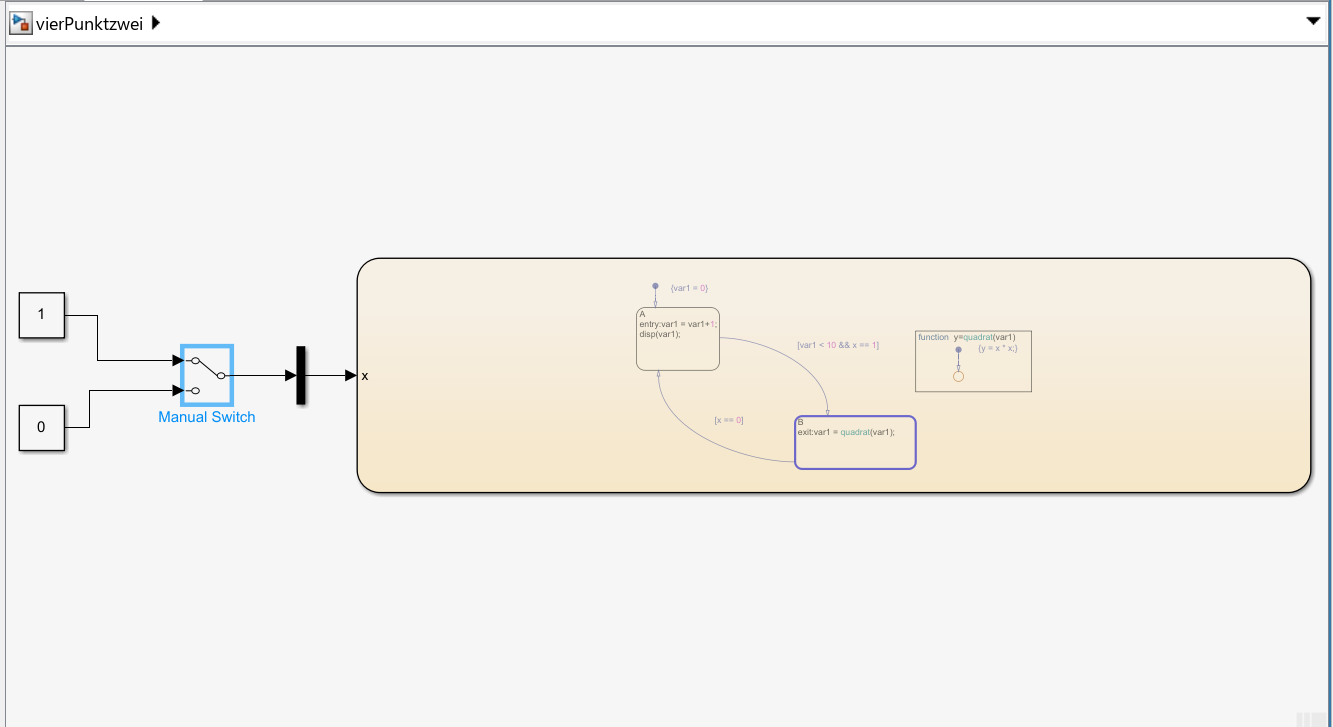
\includegraphics[scale=0.7]{Aufgabe4.3e.png}
				\caption{Nächste Erweiterung.}
				\label{fig_11: Aufg_3e}
			\end{figure}
			Bei dem bereits zusehende dritten State, handelt es sich nicht direkt um ein State, sondern um die geforderte \textit{grafische Funktion}. Dabei handelt es sich um einen separaten Stateblock, der keine Verbindungen zu den anderen States benötigt. Die Funktion wird vergleichsweise klassisch aufgerufen wie Funktionen in Java oder C/C++. \\
			In $State\ B$ wird ein Variable `var1` deklariert. Diese bekommt den Rückgabewert der aufgerufenen Funktion, hier `quadrat(var1)`, zugewiesen.
			\begin{figure}[h]
				\centering
				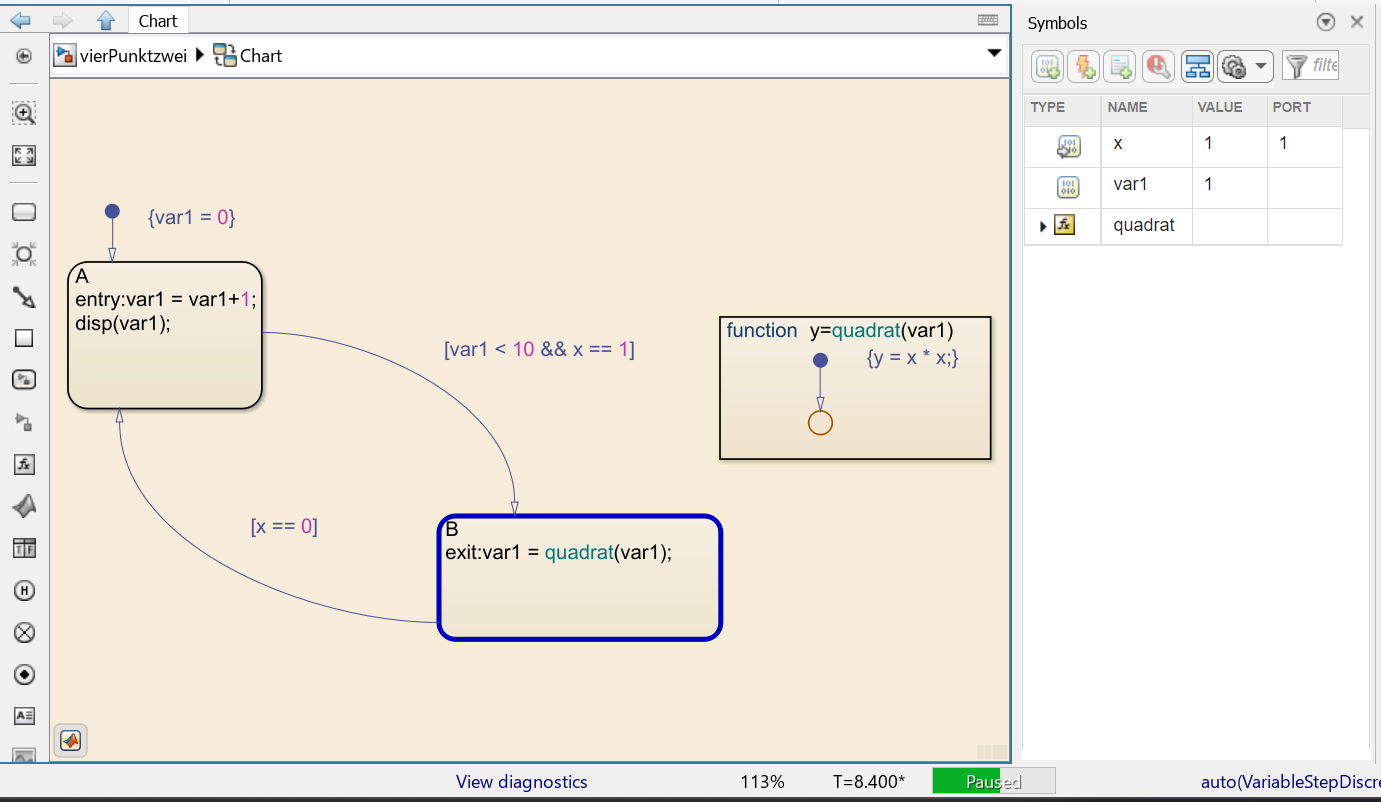
\includegraphics[scale=0.6]{Aufgabe4.3eChart.png}
				\caption{Erweiterung durch eine grafische Funktion.}
				\label{fig_12: Aufg_3e_Chart}
			\end{figure}
\clearpage
\newpage
	\section{Anwendungsbeispiel - Mischer}
		\begin{figure}[h]
			\centering
			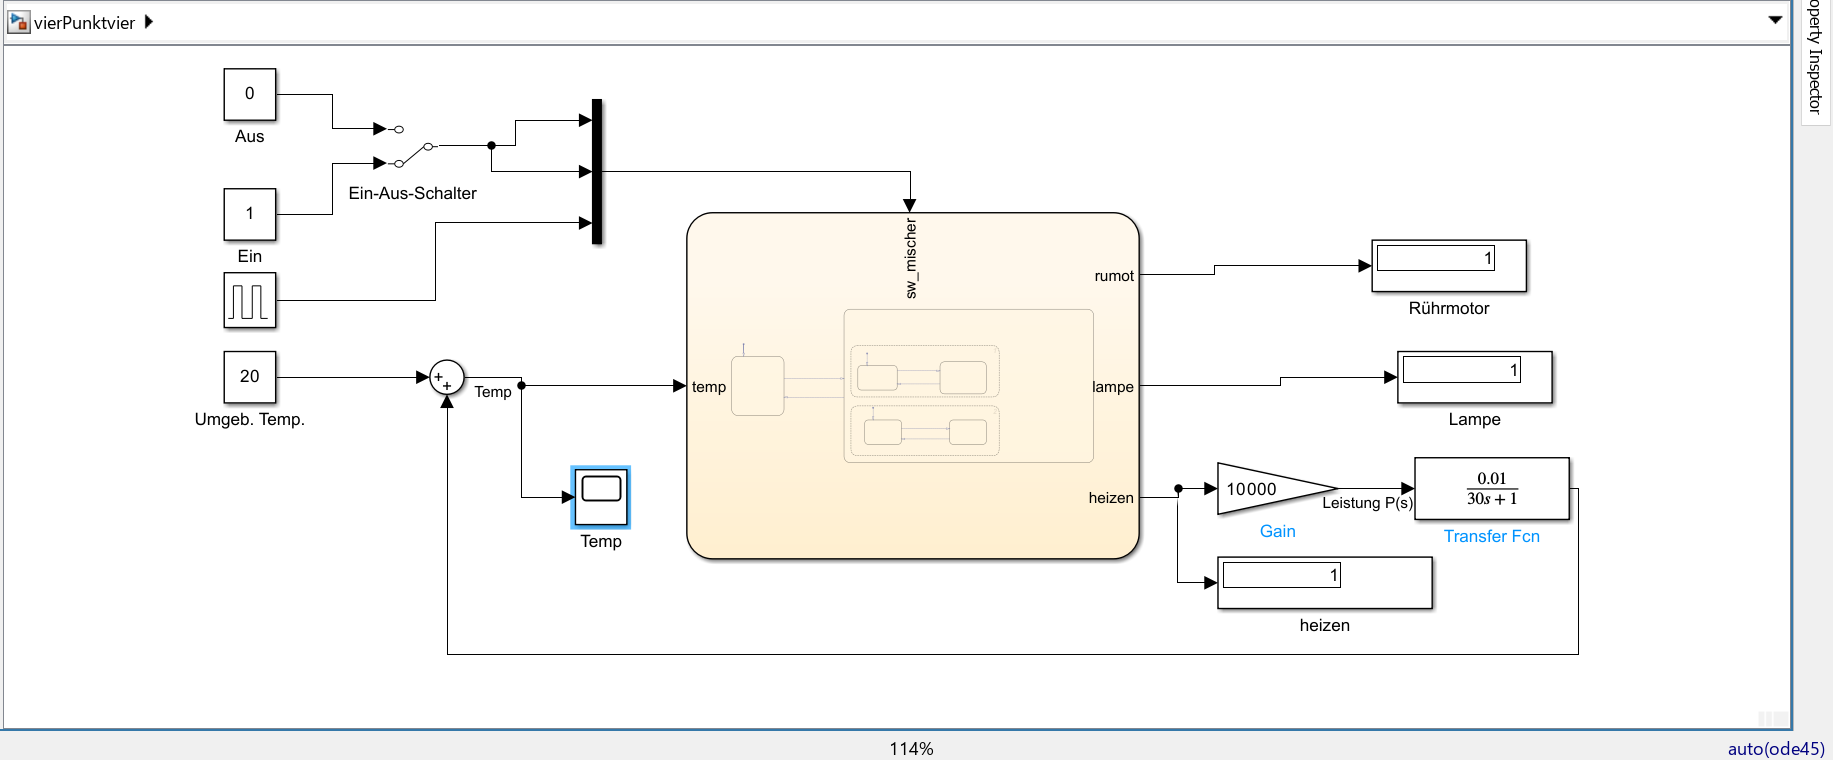
\includegraphics[scale=0.5]{Aufgabe4.4a.png}
			\caption{Simulink-Modell für den Mischer.}
			\label{fig_12: Aufg_4a_SimulinkModell}
		\end{figure}
		\subsection{}
			Aus der 1.Differntialgleichung
			$$c\cdot m \cdot \frac{d\vartheta(t)}{dt}= P(t) - O\cdot k \cdot \vartheta(t) $$
			lässt sich folgende Übertragungsfunktion erzeugen
			$$G(s) = \frac{\vartheta (s)}{P(s)}$$
			$$ = \frac{1}{c\cdot m + O\cdot k} $$
			$$ = \frac{\frac{1}{O\cdot k}}{\frac{c\cdot m}{O\cdot k}s + 1}$$
			Mit $K=\frac{1}{O\cdot k} = 1$ und $T_1 = c\cdot m \cdot k = 30 sec$ sieht die Übertragsfunktions für den Mischer so aus:
			$$G(s) = \frac{0.001}{30s + 1}$$
			Es handelt sich damit um ein PT-1-Glied.
\clearpage
		\subsection{}
			\begin{figure}[h]
				\centering
				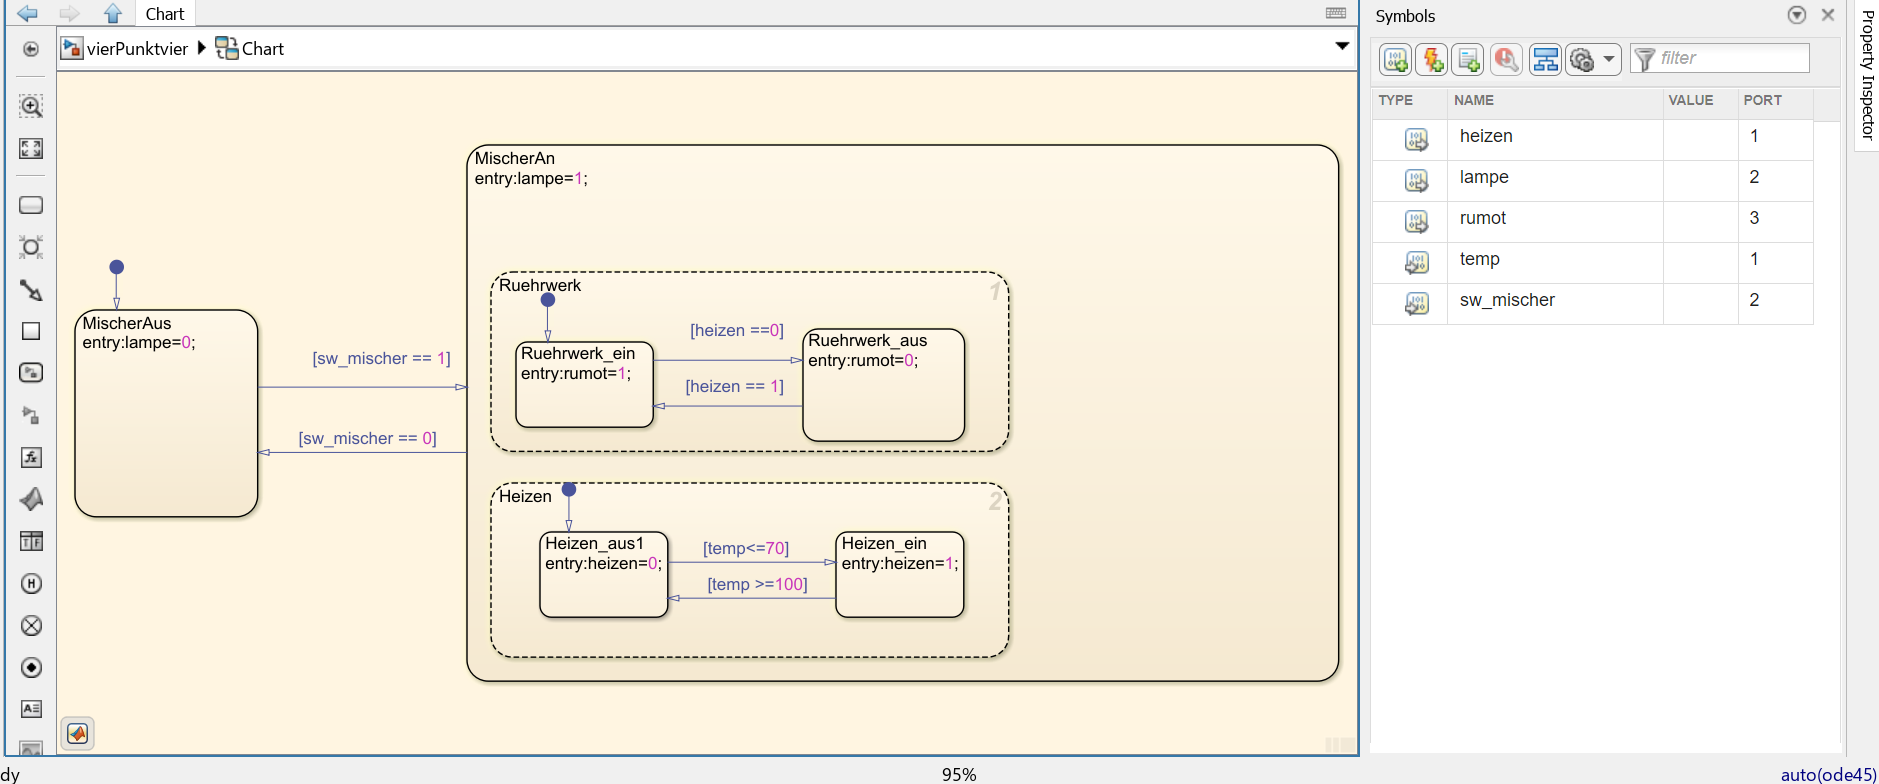
\includegraphics[scale=0.5]{Aufgabe4.4Chart.png}
				\caption{Erstelltes Chart für die Mischersteuerung.}
				\label{fig_13: Aufg_4b_Mischer}
			\end{figure}
		\subsection{}
			\begin{figure}[h]
				\centering
				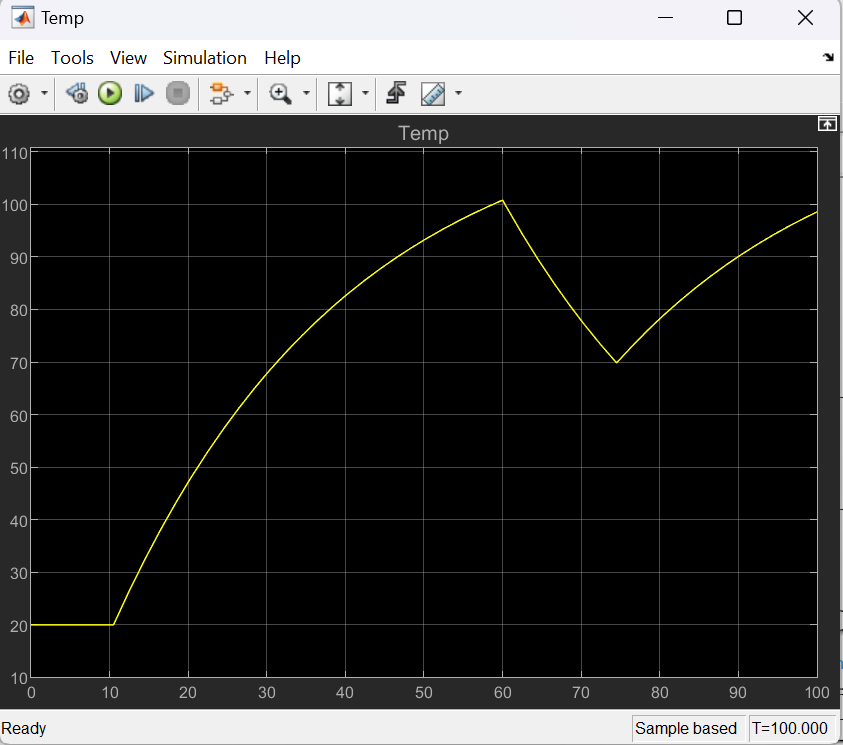
\includegraphics[scale=0.46]{Aufgabe4cTempDisplay.png}
				\caption{Der Temperaturverlauf der Heizung. Zu erkennen sind der Heizvorgang von $0 - 70$°C und das Abkühlen von $100 - 70$°C}
				\label{fig_14: Aufg_4c_TempGraph}
			\end{figure}
\clearpage
		\subsection{}
			Aus dem Graph (Abb. 14) lässt sich die Zeit sehr gut ablesen. Die Dauer des
			\begin{itemize}
				\item Heizens: $\ 49\ sec\ = 60 - 11$
				\item Abkühlen: $ 14\ sec\ = 74 - 60$
			\end{itemize}
		
\end{document}